% ------------------------------------------------------------------------------
% TYPO3 Version 10.1 - What's New (German Version)
%
% @license	Creative Commons BY-NC-SA 3.0
% @link		http://typo3.org/download/release-notes/whats-new/
% @language	German
% ------------------------------------------------------------------------------

\section{Änderungen für Integratoren}
\begin{frame}[fragile]
	\frametitle{Änderungen für Integratoren}

	\begin{center}\huge{Kapitel 2:}\end{center}
	\begin{center}\huge{\color{typo3darkgrey}\textbf{Änderungen für Integratoren}}\end{center}

\end{frame}

% ------------------------------------------------------------------------------
% Feature | 89102 | Read settings for sites from <config>/sites/<siteIdentifier>/settings.yaml
%
%\begin{frame}[fragile]
%	\frametitle{Changes for Integrators}
%	\framesubtitle{Site-specific Settings (1)}
%
%	% decrease font size for code listing
%	\lstset{basicstyle=\smaller\ttfamily}
%
%	\begin{itemize}
%		\item A YAML file can provide site specific variables independent of the current context.
%
%		\item Place the file in the site configuration folder:\newline
%			\texttt{<config>/sites/<siteIdentifier>/settings.yaml}
%
%		\item For example:
%
%\begin{lstlisting}
%Vendor:
%   MyExtension:
%      storagePid: 1
%      limit: 15
%\end{lstlisting}
%
%	\end{itemize}
%
%\end{frame}
%
% ------------------------------------------------------------------------------
% Feature | 89102 | Read settings for sites from <config>/sites/<siteIdentifier>/settings.yaml
%
%\begin{frame}[fragile]
%	\frametitle{Changes for Integrators}
%	\framesubtitle{Site-specific Settings (2)}
%
%	% decrease font size for code listing
%	\lstset{basicstyle=\smaller\ttfamily}
%
%	\begin{itemize}
%		\item Settings can be accessed in TypoScript:
%
%\begin{lstlisting}
%plugin.tx_example.storagePid = {$Vendor.MyExtension.storagePid}
%\end{lstlisting}
%
%		\item Settings can also be accessed in PHP using the \texttt{Site} object:
%
%\begin{lstlisting}
%$settings = $site->getSettings();
%$storagePid = $settings['MyVendor']['MyExtension']['storagePid'];
%\end{lstlisting}
%
%	\end{itemize}
%
%\end{frame}

% ------------------------------------------------------------------------------
% Feature | 89227 | Ask for email address while installing TYPO3

\begin{frame}[fragile]
	\frametitle{Änderungen für Integratoren}
	\framesubtitle{E-Mail-Adresse des Administrators}

	\begin{columns}[T]
		\begin{column}{.04\textwidth}
		\end{column}
		\begin{column}{.38\textwidth}

			Während des Installationsvorgangs kann jetzt eine E-Mail-Adresse eingegeben werden.
			Diese Adresse wird für den initialen Admin Backend-Benutzer verwendet.

			\vspace{0.2cm}

			Die selbe Option gibt es im Wartungsmodul
			\textbf{Create Administrative User} des Install Tools.

		\end{column}
		\begin{column}{.58\textwidth}
			\vspace{-0.3cm}
			\begin{figure}
				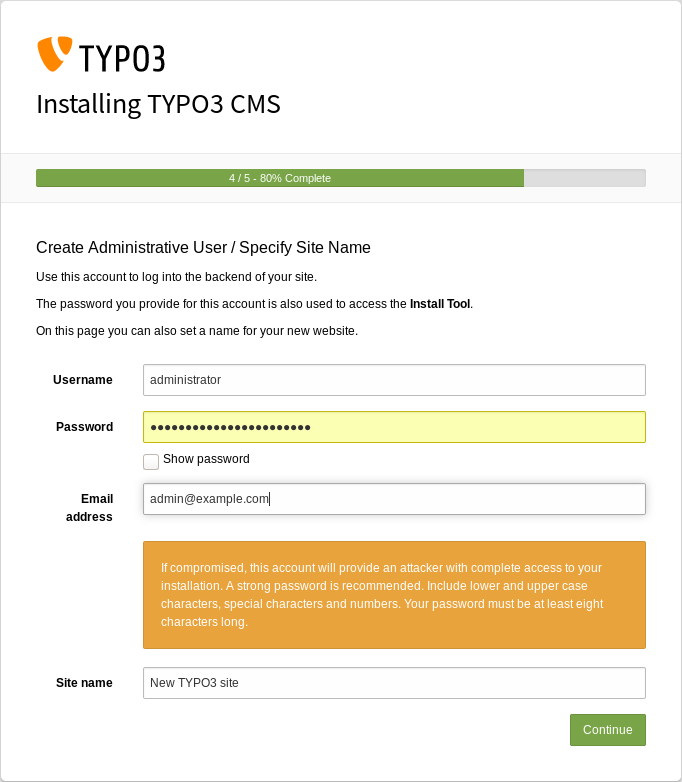
\includegraphics[width=0.70\linewidth]{ChangesForIntegrators/89227-EmailAddressDuringInstallation.png}
			\end{figure}
		\end{column}
	\end{columns}

\end{frame}

% ------------------------------------------------------------------------------
% Feature | 89229 | Cache Preset for Settings in Maintenance Area

% TRANSLATORS, PLEASE BE AWARE:
% We already included this slide in the 10.0 What's New Slides! However, the
% feature #89229 was removed from the TYPO3 core shortly before version 10.0 was
% published. Therefore, you possibly don't need to translate this slide again
% (just copy the text from the previous What's New Slides (search for the term
% "Cache Storage Type" in file ChangesForIntegrators.tex).

\begin{frame}[fragile]
	\frametitle{Änderungen für Integratoren}
	\framesubtitle{Cache Speichertyp (1)}

	\begin{itemize}

		\item TYPO3 verfügt über ein flexibles Caching-System mit einer Standardkonfiguration,
			die für die meisten Anwendungsfälle ideal ist.
		\item Der Speichertyp kann nun auch konfiguriert werden,  um die Caches zu optimieren 
			und die Leistung je nach individueller Umgebung zu erhöhen.

			\begin{itemize}
				\item Wählen Sie den Speicher \textbf{database} für eine Standardumgebung aus
					oder wenn beispielsweise ein Netzwerkdateisystem (NFS) verwendet wird.
				\item Wählen Sie \textbf{file system} wenn zum Beispiel eine verteilte 
					Datenbankeinrichtung verwendet wird.
				\item Wählen Sie \textbf{custom cache settings} um den Speichertyp für jeden Cache 
					individuell zu konfigurieren.
			\end{itemize}

		\item Bei komplexeren Installationen und speicherbasierten Caches sollten zum Beispiel 
			\href{https://redis.io/}{Redis}
			oder
			\href{https://memcached.org/}{Memcached}
			berücksichtigt werden.

	\end{itemize}

\end{frame}

% ------------------------------------------------------------------------------
% Feature | 89229 | Cache Preset for Settings in Maintenance Area

% TRANSLATORS, PLEASE BE AWARE:
% We already included this slide in the 10.0 What's New Slides! However, the
% feature #89229 was removed from the TYPO3 core shortly before version 10.0 was
% published.
%
% On this slide, the path to the function in the backend needs to be adjusted:
% ADMIN TOOLS -> Settings -> Configuration Presets

\begin{frame}[fragile]
	\frametitle{Änderungen für Integratoren}
	\framesubtitle{Cache Speichertyp (2)}

	\begin{itemize}

		\item Backend: \textbf{ADMIN TOOLS} \ding{223}\hspace{0.1cm}\textbf{Einstellungen} \ding{223}\hspace{0.1cm}\textbf{Konfigurationsvoreinstellungen}:
	\end{itemize}

	\begin{figure}
		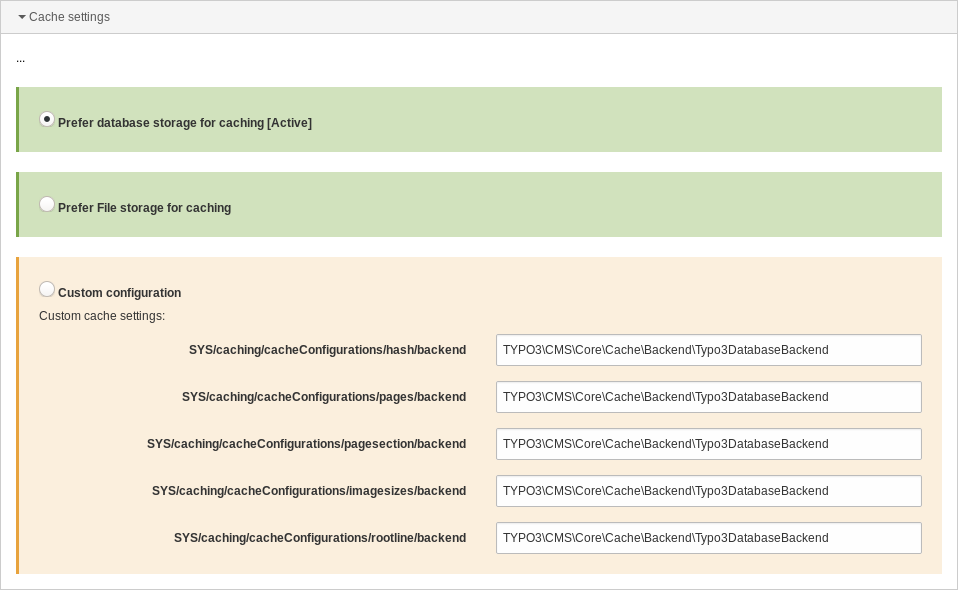
\includegraphics[width=0.60\linewidth]{ChangesForIntegrators/89229-CachePresetForSettingsInMaintenanceArea.png}
	\end{figure}

\end{frame}

% ------------------------------------------------------------------------------
% Feature | 89142 | Create site configuration if page is created on root level

\begin{frame}[fragile]
	\frametitle{Änderungen für Integratoren}
	\framesubtitle{Site-Konfiguration}

	\begin{itemize}
		\item Wenn eine neue Seite auf Root Level erstellt wird, wird damit automatisch
			eine Standard-Site-Konfiguration generiert.
		\item Demzufolge kann eine grundlegende TYPO3-Site schnell aufgesetzt werden.
		\item Die Site-Konfigurationsfunktionen:

			\begin{itemize}
				\item eine vordefinierte Identifier (e.g. \texttt{site-42-a1d0c6e83f})
				\item ein Einstiegspunkt (e.g. \texttt{https://example.com/site-42})
				\item eine default Sprache (e.g. \texttt{Englisch})
			\end{itemize}

	\end{itemize}

\end{frame}

% ------------------------------------------------------------------------------
% Feature | 89090 | Reports for conflicting redirects

\begin{frame}[fragile]
	\frametitle{Änderungen für Integratoren}
	\framesubtitle{Konflikte bei Redirects (1)}

	\begin{itemize}
		\item Ein neuer Symfony-Befehl wurde eingeführt, um Weiterleitungen zu erkennen,
			die mit Seiten-URLs in Konflikt stehen.
		\item Führen Sie den Befehl in der CLI aus:\newline
			\smaller
				(Der optionale Parameter \texttt{-}\texttt{-site} begrenzt die Prüfung auf eine bestimmte Seite)
			\normalsize
	\end{itemize}

	\begin{figure}
		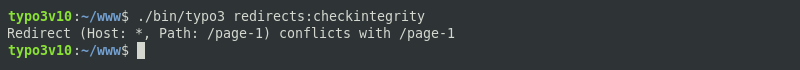
\includegraphics[width=0.90\linewidth]{ChangesForIntegrators/89090a-ReportsForConflictingRedirects.png}
	\end{figure}

	\begin{itemize}
		\item Der Befehl ist auch als Scheduler-Task verfügbar:
	\end{itemize}

	\begin{figure}
		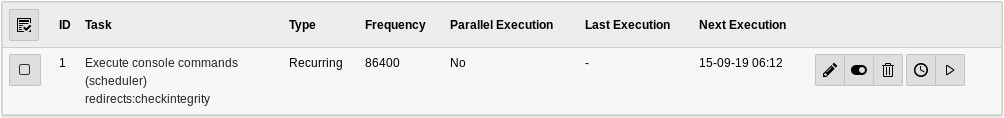
\includegraphics[width=0.90\linewidth]{ChangesForIntegrators/89090b-ReportsForConflictingRedirects.png}
	\end{figure}

\end{frame}

% ------------------------------------------------------------------------------
% Feature | 89090 | Reports for conflicting redirects

\begin{frame}[fragile]
	\frametitle{Änderungen für Entwickler}
	\framesubtitle{Konflikte bei Redirects (2)}

	\begin{itemize}
		\item Im Modul Berichte kann auch eine Liste widersprüchlichen Weiterleitungen zugegriffen werden:
	\end{itemize}

	\begin{figure}
		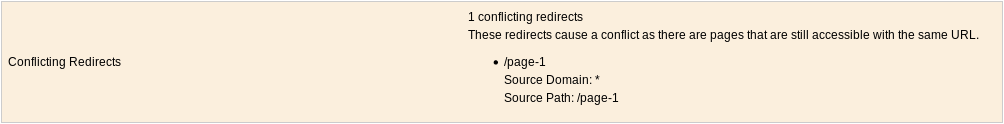
\includegraphics[width=0.90\linewidth]{ChangesForIntegrators/89090c-ReportsForConflictingRedirects.png}
	\end{figure}

	\begin{itemize}
		\item
			\small\textbf{Anmerkung:}
				Der Befehl muss erneut ausgeführt werden, um die Liste 'zurückzusetzen'.
				Durch Beheben des Problems (z.B. durch Entfernen der Weiterleitung) wird die Liste nicht geleert.
			\normalsize
	\end{itemize}

\end{frame}

% ------------------------------------------------------------------------------
% Feature | 89010 | Introduce Site Configuration for Distribution Packages

\begin{frame}[fragile]
	\frametitle{Änderungen für Integratoren}
	\framesubtitle{Distributionspakete}

	% decrease font size for code listing
	\lstset{basicstyle=\tiny\ttfamily}

	\begin{itemize}
		\item Distributionen können jetzt Site-Konfigurationsdateien bereitstellen.

		\item Erstellen Sie ein Verzeichnis/eine Datei im Distributionspaket wie folgt:\newline
			\texttt{Initialisation/Site/<siteIdentifier>/config.yaml}

		\item Ähnlich wie bei Assets, die nach \texttt{fileadmin/} verschoben werden,\newline
			werden Standardkonfigurationen in den Ordner \texttt{config/} verschoben.

		\item Wenn das Zielverzeichnis bereits vorhanden ist, wird keine Änderung an der vorhandenen Konfiguration vorgenommen.
	\end{itemize}

\end{frame}

% ------------------------------------------------------------------------------
% Feature | 88318 | Display Application Context in CLI

\begin{frame}[fragile]
	\frametitle{Änderungen für Integratoren}
	\framesubtitle{Application Context in CLI}

	\begin{itemize}
		\item Der aktuelle Application Context wird nun in CLI-Anforderungen neben der 
			TYPO3-Versionsnummer angezeigt:
	\end{itemize}

	\begin{figure}
		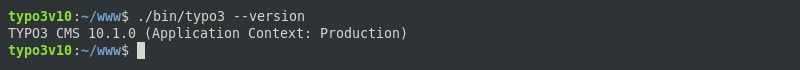
\includegraphics[width=0.90\linewidth]{ChangesForIntegrators/88318-DisplayApplicationContextInCli.png}
	\end{figure}

\end{frame}

% ------------------------------------------------------------------------------
% Feature | 87525 | Add api=1 option in VimeoRenderer

\begin{frame}[fragile]
	\frametitle{Änderungen für Integratoren}
	\framesubtitle{Vimeo Video-Rendering}

	% decrease font size for code listing
	\lstset{basicstyle=\smaller\ttfamily}

	\begin{itemize}
		\item Der Parameter \texttt{api=1} in Vimeo-Video-URLs ermöglicht API-Interaktionen mit dem Videoplayer (z.B. Hinzufügen von Schaltflächen zur Steuerung des Videos).
		\item Integratoren können diesen Parameter jetzt auf zwei verschiedene Weisen einstellen:

		\begin{itemize}
			\item Mit TypoScript:

\begin{lstlisting}
lib.contentElement.settings.media.additionalConfig.api = 1
\end{lstlisting}

			\item In Fluid, mit Media-ViewHelper:

\begin{lstlisting}
<f:media
  file="{file}"
  alt="{file.properties.alternative}"
  title="{file.properties.title}"
  additionalConfig="{api: 1}"
/>
\end{lstlisting}

		\end{itemize}
	\end{itemize}

\end{frame}

% ------------------------------------------------------------------------------
% Feature | 86670 | Make default action in DragUploader adjustable

\begin{frame}[fragile]
	\frametitle{Änderungen für Integratoren}
	\framesubtitle{Hochladen von Dateien}

	% decrease font size for code listing
	\lstset{basicstyle=\smaller\ttfamily}

	\begin{itemize}
		\item Es ist jetzt möglich, die Standardaktion beim Hochladen von Dateien im Dateilistenmodul durch Drag and Drop zu konfigurieren.
		\item Benutzer TSConfig:

\begin{lstlisting}
# Set default to replace:
options.file_list.uploader.defaultAction = replace

# Set default to rename:
options.file_list.uploader.defaultAction = rename

# Set default to cancel:
options.file_list.uploader.defaultAction = cancel
\end{lstlisting}

	\end{itemize}

\end{frame}

% ------------------------------------------------------------------------------
% Feature | 84250 | Separately enable / disable "Add media by URL" and "Select & upload files"

\begin{frame}[fragile]
	\frametitle{Änderungen für Integratoren}
	\framesubtitle{Tasten für Medienelemente}

	% decrease font size for code listing
	\lstset{basicstyle=\tiny\ttfamily}

	\begin{itemize}
		\item Die Tasten \textbf{"Add media by URL"} und \textbf{"Select \& upload files"}
			können nun unabhängig voneinander aktiviert/deaktiviert werden.
	\end{itemize}

	\begin{figure}
		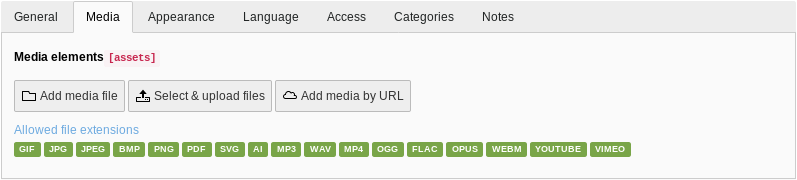
\includegraphics[width=0.75\linewidth]{ChangesForIntegrators/84250-EnableDisableMediaButtons.png}
	\end{figure}

	\begin{itemize}
		\item Im folgenden Beispiel werden beide Tasten ausgeblendet:

\begin{lstlisting}
$GLOBALS['TCA']['pages']['columns']['media']['config']['appearance'] = [
  'fileUploadAllowed' => false,
  'fileByUrlAllowed' => false,
];
\end{lstlisting}

	\end{itemize}

\end{frame}

% ------------------------------------------------------------------------------
% Feature | 88441 | Show configuration of USER_INT objects in adminpanel

\begin{frame}[fragile]
	\frametitle{Änderungen für Integratoren}
	\framesubtitle{Admin-Panel}

	\begin{itemize}
		\item Der Admin-Panel enthält ein neues Panel \textbf{USER\_INT} unter dem Modul 'Info'.
	\end{itemize}

	\begin{figure}
		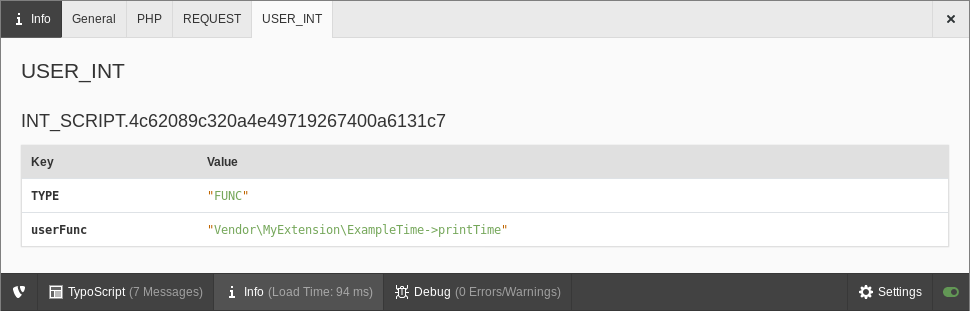
\includegraphics[width=0.90\linewidth]{ChangesForIntegrators/88441-ShowUserIntObjectsInAdminPanel.png}
	\end{figure}

\end{frame}

% ------------------------------------------------------------------------------
